%---------------------------------------------------
% کلاس سند: article برای اسناد متنی، با اندازه کاغذ A4 و فونت پایه 16
\documentclass[a4paper,16pt]{article}

% بسته‌های ریاضی برای معادلات و نمادهای پیشرفته
\usepackage{amsmath, amssymb, amstext}

% بسته رنگ برای استفاده از رنگ در متن یا محیط‌ها
\usepackage{xcolor}

% بسته گرافیک برای درج تصاویر
\usepackage{graphicx}

% تنظیمات حاشیه صفحه
\usepackage{geometry}

% بسته لینک‌دهی (هایپرلینک‌ها)
\usepackage{hyperref}

% بسته صفحه‌آرایی برای تنظیم هدر و فوتر
\usepackage{fancyhdr}


% بسته xepersian برای پشتیبانی از زبان فارسی با XeLaTeX
\usepackage{xepersian}

% تعیین فونت فارسی (فایل فونت باید موجود باشد یا در سیستم نصب باشد)
\settextfont{BNAZANIN.TTF}

% تنظیم اندازه حاشیه‌ها از هر طرف برابر با 1 اینچ
\geometry{margin=1in}

% تنظیم سبک fancy برای سربرگ و پاورقی
\pagestyle{fancy}

% سمت چپ هدر: مشخص‌کننده سری تمرین و نام درس
\lhead{تمرین سری یک درس مکانیک تحلیل }

% وسط هدر: نام دانشکده
\chead{دانشکده فیزیک دانشگاه صنعتی خواجه نصیرالدین طوسی}

% سمت راست هدر: تاریخ روز به‌صورت خودکار
\rhead{\today}

% پایین صفحه: شماره صفحه
\cfoot{\thepage}

% شروع سند
\begin{document}
	
	% صفحه عنوان (بدون هدر و فوتر)
	\thispagestyle{empty}
	\begin{center}
		% لوگوی دانشگاه (باید فایل تصویر در مسیر پروژه باشد)
		
\includegraphics[width=0.5\textwidth]{../../images/image-E_1/image-1.png} \\[10pt] 
		
		% عنوان سند
		\textbf{\LARGE عنوان:تمرین سری‌یک}\\[20pt]
		
		% نیم‌سال تحصیلی
		\textbf{\LARGE نیم‌سال تحصیلی:4041 }\\[10pt]
		
		% نام مدرس درس
		\textbf{\Large مدرس: دکتر محمد انصاری‌فرد}\\[10pt]
		
		% مبحث تمرین 
		\textbf{\Large مبحث تمرین:مروری بر فیزیک پایه   }\\[10pt]
		
		% مهلت تحویل تمرین
		\textbf{\Large مهلت تحویل:14مهر }
	\end{center}
	
	% صفحه جدید برای ادامه سند
	\newpage
	
	% ایجاد فهرست مطالب به‌صورت خودکار (براساس \section و \subsection و ...)
	\tableofcontents
	\newpage
	
	
	\section{سوال اول}
	جرم جسمی با زمان طبق رابطه زیر تغییر می‌کند:
	\[
	m(t) = m_0 e^{-\alpha t}
	\]
	که در آن $\alpha$ یک ثابت است. جرم جسم در لحظه $t=0$ برابر $m_0$ است.  
	اگر سرعت جسم در لحظه $t=0$ برابر $v_0$ باشد و هیچ نیروی خارجی به جسم وارد نشود،  
	سرعت آن در لحظه $t$ چگونه خواهد بود؟
	\\
	راهنمایی:دید ‌ریاضی به این مورد داشته باشید(دنبال شهود فیزیکی نگردید.)

	\section{سوال دوم}

	متحرکی بر روی محور $x$ حرکت می‌کند.  
	رابطه بین مکان و زمان این متحرک به صورت زیر است:
	\[
	t = a x^2 + b x + 1
	\]
	که در آن $a$ و $b$ مقادیر ثابتی هستند.شتاب این متحرک کدام است؟
	\section{سوال سوم}
	
	گویی به جرم $M$ بر روی یک سطح افقی قرار دارد.گوی می‌تواند روی سطح بلغزد و ارتفاع ضلع قائم آن برابر با $H$ است.مطابق شکل، جسم کوچکی به جرم $m=\alpha M$ بر روی سطح افقی با سرعت اولیه $v$ به سمت گوی حرکت می‌کند.کمترین مقدار $v$ چقدر باشد تا جسم کوچک به بالای گوی برسد؟(تمام سطوح بدون اصطکاک هستند و $\alpha$ مقداری ثابت است.)  
	\begin{figure}[h]
	    \centering
	    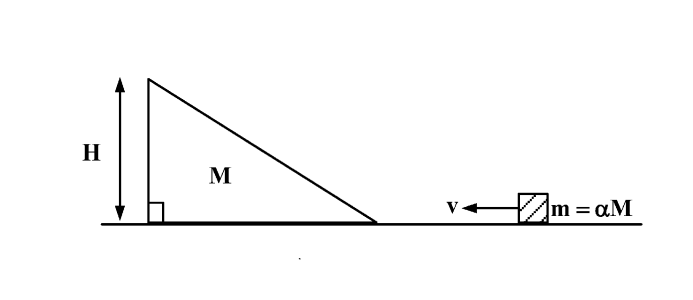
\includegraphics[width=0.5\textwidth]{../../images/image-E_1/image-3.png}
	    \caption{}
	    \label{fig:square_particles}
	\end{figure}
	
	\section{سوال چهارم}
	
	دو جرم $m$ و $M=3m$ به دو انتهای یک ریسمان سبک بسته شده‌اند.ریسمان از روی یک قرقره ثابت، بدون جرم و بدون اصطکاک، عبور می‌کند، به گونه‌ای که $m$ و $M$ در دو طرف قرقره آویزان هستند.سیستم را از حال سکون رها می‌کنیم:
	\\
	الف) شتاب هرکدام از جسم هارا بدست آورید.
	\\
	ب) نیروی وارد بر ریسمان  را بدست آورید.  
	\\
	ج)اندازه شتاب مرکز جرم این سیستم کدام است؟
		\begin{figure}[h]
		\centering
		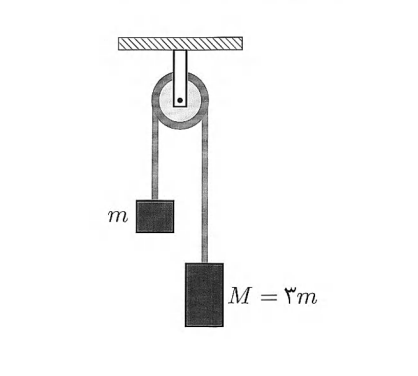
\includegraphics[width=0.5\textwidth]{../../images/image-E_1/image-2.png}
		\caption{}
		\label{fig:square_particles}
	\end{figure}
	\newpage
	\section{سوال پنجم}
	
	معادله حرکت ذره‌ای به جرم $m$ که در راستای $x$ حرکت می‌کند، به صورت زیر است:
	\[
	x =-t+2t^{3}
	\]
	که در آن $x$ بر حسب متر و زمان بر حسب ثانیه است.توانی که در لحظه $t = 2$ ثانیه به این ذره منتقل می‌شود، چند وات است؟
	\section{سوال ششم}
فرض کنید دو بردار زیر در فضای سه‌بعدی داده شده‌اند:
\[
\mathbf{A} = (1,\,2,\,3) , \quad \mathbf{B} = (2,\, -1,\, 1)
\]

\begin{itemize}
	\item[$\square$]ضرب داخلی \(\mathbf{A} \cdot \mathbf{B}\) را محاسبه کنید.  
	\item[$\square$] ضرب خارجی (برداری) \(\mathbf{A} \times \mathbf{B}\) را به دست آورید.  
	\item[$\square$]اگر \(\mathbf{C} = (0,\,1,\, -1)\)، ضرب سه‌گانه‌ی \(\mathbf{A} \cdot (\mathbf{B} \times \mathbf{C})\) را محاسبه کنید.  
	\item[$\square$] بررسی کنید آیا بردارهای \(\mathbf{A}, \mathbf{B}, \mathbf{C}\) در یک صفحه قرار دارند یا خیر.  
\end{itemize}
\section{سوال امتیازی}

ثابت کنید که برای هر سه بردار $\mathbf{A},\mathbf{B},\mathbf{C}\in\mathbb{R}^3$، رابطه زیر برقرار است:
\[
\boxed{\;\mathbf{A}\times(\mathbf{B}\times\mathbf{C})
	=\mathbf{B}(\mathbf{A}\cdot\mathbf{C})-\mathbf{C}(\mathbf{A}\cdot\mathbf{B})\;}
\]
	\vspace{10pt}
\textbf{موفق باشید.}
\end{document}
